\documentclass[14pt]{extarticle}

% Esto es para poder escribir acentos directamente:
\usepackage[utf8]{inputenc}
% Esto es para que el LaTeX sepa que el texto est en espaol:
\usepackage[spanish, activeacute]{babel}

% Paquetes de la AMS:
\usepackage{amsmath, amsthm, amsfonts}

\usepackage{extsizes}

\usepackage{pdflscape}
\usepackage{fontawesome}

\usepackage{graphicx}
\graphicspath{ {./images/} }

\usepackage[margin=1in]{geometry}

\usepackage{listings}
\usepackage{natbib}
\usepackage{url}
\usepackage{hyperref} % For hyperlinks in the PDF
\usepackage{multirow}
\usepackage{xifthen}
\usepackage{tabularx}

% Teoremas
%--------------------------------------------------------------------------
\newtheorem{thm}{Teorema}[section]
\newtheorem{cor}[thm]{Corolario}
\newtheorem{lem}[thm]{Lema}
\newtheorem{prop}[thm]{Proposicin}
\theoremstyle{definition}
\newtheorem{defn}[thm]{Definicin}
\theoremstyle{remark}
\newtheorem{rem}[thm]{Observacin}

% Atajos.
% Se pueden definir comandos nuevos para acortar cosas que se usan
% frecuentemente. Como ejemplo, aqu se definen la R y la Z dobles que
% suelen representar a los conjuntos de nmeros reales y enteros.
%--------------------------------------------------------------------------

\def\RR{\mathbb{R}}
\def\ZZ{\mathbb{Z}}

% Operadores.
% Los operadores nuevos deben definirse como tales para que aparezcan
% correctamente. Como ejemplo definimos en jacobiano:
%--------------------------------------------------------------------------
\DeclareMathOperator{\Jac}{Jac}

%--------------------------------------------------------------------------
%\title{Práctica 1 \\  Navegación de robots y arquitecturas de control}
%\author{Javier Moreno}
\begin{document}
%\maketitle
\begin{titlepage}

\begin{center}
\vspace*{-1in}
\begin{figure}[htb]
\begin{center}

\includegraphics{upm.jpg}
\end{center}
\end{figure}
MÁSTER UNIVERSITARIO EN INTELIGENCIA ARTIFICIAL\\
\vspace*{0.15in}
DEPARTAMENTO DE INTELIGENCIA ARTIFICIAL \\
\vspace*{0.6in}
\begin{large}
ROBOTS AUTÓNOMOS\\
\end{large}
\vspace*{0.2in}
\begin{Large}
\textbf{PRÁCTICA 1: NAVEGACIÓN DE ROBOTS Y ARQUITECTURAS DE CONTROL} \\
\end{Large}
\vspace*{0.3in}
\begin{large}
JAVIER MORENO VEGA\\
\end{large}
\vspace*{0.3in}
\rule{80mm}{0.1mm}\\
\vspace*{0.1in}
\today
\end{center}
\end{titlepage}
\newpage
\tableofcontents % índice de contenidos
\cleardoublepage
\section{Introducción}\label{sec:introduccion}
\textit{Navegación de robots es la metodología que permite guiar el curso de un robot móvil a través de un entorno con obstáculos. }\cite{pdf:navegacion_de_robot}
\\\\Como bien definía esta práctica, era una introducción al software V-Rep para la navegación con robots sobre el robot Pioneer-3DX, empezando con un controlador reactivo e intentando trabajar con aprendizaje con refuerzo.\\
\begin{center}
	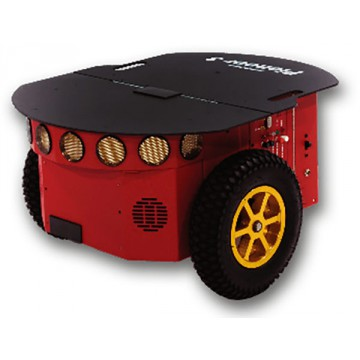
\includegraphics[scale=0.6]{pioneer.jpg}
\end{center}
\begin{center}
	[Imagen 1: Robot Pioneer-3DX]
\end{center}
La práctica se empezó con un controlador muy sencillo que solo evitaba los obstáculos, y se fue iterando sobre él hasta conseguir uno "más avanzado" que seguía un corredor y terminaba al detectar el fina, tal y como pedía el enunciado de esta práctica. Se han creado varios mundos para experimentar con este controlador, como se enseñará en los experimentos.\\\\
Para el final de la práctica se ha investigado sobre el aprendizaje por refuerzo \cite{pdf:reinforcementlearning} con el fin de que fuera el propio agente el que creara su controlador al explorar el entorno. Se presenta una versión preliminar con una idea para trabajar en mundos continuos usando Q-learning \cite{pdf:qlearning1} \cite{pdf:qlearning2} y el Proceso de Decisión de Markov (MDP).
\section{Instalación y arquitectura creada}\label{sec:instalacionyarquitecturacreada}
La instalación del software no tuvo ningún problema complicado, lo único que costó mas detectar fue que había que darle permisos de ejecución al script Python client. Esta instalación se ha realizado sobre un sistema Xubuntu 16.0xx con kernel xxx, V-Rep xxx y python xxx. Además sobre un portatil Macbook Pro 2017 macOS High Sierra 10.13, V-Rep  Pro Edu 3.4.0 y python 2.7.10.\\\\
Acerca de la arquitectura seguida, se ha intentado modularizar todo lo posible para evitar scripts demasiado largos y confusos. Se ha creado una clase llamada RemoteConnection que es la encargada de gestionar la conexión con V-Rep, recibe en el constructor los argumentos de llamada (puerto, los manejadores de los motores y el robot, etc) y crea una instancia RemoteConnection. Esta clase es la que iniciar el controlador, el cuál es pasado a través de otro script como argumento del método de RemoteConnection "run". Por lo tanto desde el controlador no es necesario llamar a ninguna función de V-Rep, sólo se llaman a métodos ya creados de RemoteConnection, y esta es la que llama a V-Rep. Además se encarga de la gestión de errores y de escribir mensajes de log en la consola de V-Rep.\\\\
Cada controlador, o versión de este, se escribe en archivos diferentes, sin hacer ninguna llamada, esta se realiza desde client.py, el cual realiza el import del controlador a utilizar, llama al constructor y al método run.\\\\
Aunque en la versión de prueba dada por el profesor los sensores se pasaban como argumentos desde el script del servidor de V-Rep, he preferido llamar a los sensores desde los script remotos en python.\\\\
Para los experimentos se han creado tres mundos, a parte del dado por el profesor (y modificado un poco).\\\\
\newpage
\textbf{Clase RemoteConnection}\\\\
\begin{tabular}{|c|c|c|}
\hline 
Método & Devuelve & Descripción \\ 
\hline 
init & Instancia & Constructor \\ 
\hline 
run(controller) & void & Inicializador de la simulación \\ 
\hline 
printMessage(message) & int & Mensaje en consola V-Rep \\ 
\hline 
readASensor(sensor) & float & Valor de proximidad de un sensor \\ 
\hline 
readAllSensor(numberOfSensors) & array & Valores de proximidad \\ 
\hline 
getConnectionId() & int & Obtiene la conexión \\ 
\hline 
setLeftMotorVelocity(velocity) & void & Define la velocidad \\ 
\hline 
setRightMotorVelocity(velocity) & void & Define la velocidad \\ 
\hline 
getAngle() & float & Ángulo del robot \\ 
\hline 
getPosition() & array & Posición del robot \\ 
\hline 
getSensorAngle(sensorName) & float & Ángulo de un sensor \\ 
\hline 
setAngle(angle) & void & Define el nuevo ángulo del robot \\ 
\hline 
isConnectionEstablished() & bool & Conexión establecida \\ 
\hline 
\end{tabular} 
\newpage
\section{Controlador reactivo}\label{sec:controladorreactivo}
Un controlador reactivo usado sobre un agente es aquel que dependiendo de una entrada (sensor) decide una acción u otra, sin aprender de ella. Es decir, acción-reacción, siendo la reacción la proximidad a algún obstáculo.\\\\
Se han desarrollado tres versiones de un controlador reactivo, siendo la primera la más simple, y la última una funcional y que cumple con los requisitos de la práctica. Voy a explicar las tres versiones y enseñar los tres mundos usados para los experimentos.
\subsection{Primera versión}\label{subsec:primeraversion}
Este controlador es el más sencillo, la base es un límite de proximidad definido, además se definen una velocidad base, una velocidad de giro y una variable de control de rotación.\\\\
 En cada iteración del controlador, y con un tiempo de pausa, se obtienen los valores de todos los sensores delanteros (sensor 1 a 8). Sobre estos valores se comprueba si hay alguno que detecte una distancia inferior al límite de proximidad definido, y sí es así se genera un giro al lado contrario de donde esté ese sensor, es decir, si es un sensor de la izquierda (1 a 4) gira a la derecha, y si es un sensor de la derecha  gira a la izquierda. Cuando se define el giro se activa la variable de rotación, la cuál no se desactivara hasta que ningún sensor tenga una proximidad inferior al límite, mientras esta variable esté activada el robot estará girando.
\subsection{Segunda versión}\label{subsec:segundaversion}
En la segunda versión del controlador reactivo se ha intentado añadir algunas mejoras: eliminar giros muy grandes, y añadir aleatoriedad sobre el ángulo.\\\\
Aunque la mejora principal es el método "setAngle", cuando empecé a trabajar en la primera versión me di cuenta que definir los giros era algo muy "prueba y error", así que para esta segunda versión me puse a trabajar en alguna forma de poder definir el giro exacto que quería y así evitar obstáculos con un giro bien definido. También implementé métodos para obtener el ángulo actual del robot y los ángulos de los sensores, y así poder girar hacia el sensor que quisiera. Esta es la base de esta versión y la final.\\\\
Como en la primera versión el controlador define varias variables de uso, las mismas que en la versión anterior y añade una velocidad máxima, una mínima y un límite de proximidad para la parte frontal. Este controlador se ejecuta también mientras la conexión esté activa y además añade una variable de control por si se termina la simulación desde el propio controlador (llega al final).\\\\
En cada iteración se obtienen los valores de los sensores delanteros y se comprueba que ninguno devuelva una proximidad inferior al límite, si es así se comprueba que el sensor que tenga esta proximidad sean los delanteros frontales (4 o 5), si no se obtiene el ángulo de este sensor y una uniforme entre -10 y +10, definiendo esta variación en el ángulo del robot (ángulo del sensor +(-) 10).\\\\
En el caso que ningún sensor supere el límite pero que los sensores frontales superen el límite proximidad frontal, se obtiene el sensor que tenga mayor proximidad (más distancia a cualquier obstáculo). Si esta proximidad es 1 (proximidad que se devuelve cuando el sensor supera su límite de detección), se selecciona aleatoriamente un sensor de todos los que tengan proximidad 1, obtiene el ángulo del sensor seleccionado y se genera una uniforme entre 0 y el ángulo, definiendo en el robot este nuevo ángulo.\\\\
Por último tenemos el caso de que no se supere ningún límite. Entonces si la velocidad actual es menor que la máxima y ningún sensor detecta obstáculo (todos devuelven 1) se aumenta la velocidad en 0.1. En cambio si la velocidad es mayor que la velocidad mínima y algún sensor detecta obstáculo (el menor no es 1) se reduce la velocidad en 0.1.
\subsection{Versión final}\label{subsec:versionfinal}
Esta versión final es una modificación de la anterior y que cumple con los requisitos de la práctica, navegar por un corredor y pararse al detectar el final.\\\\
La modificación es eliminar aún más los giros grandes e ir girando lentamente si fuera necesario. Por lo tanto se ha eliminado el segundo caso de la versión anterior (cuando superaba el límite de proximidad frontal), y el primer caso se mantiene igual excepto porque ahora se ha definido un intervalo de giro, si es un sensor de la izquierda -5 y +5 si es un sensor de la derecha; este intervalo se calcula además con una uniforme entre 0 y el mismo, y es el ángulo que se define.\\\\El último caso es igual que en la version anterior.
\subsection{Experimentos}\label{subsec:experimentos}
Se han realizado experimentos sobre tres escenarios, uno el dado por el profesor modificado añadiendo más obstáculos; y dos nuevos diseñados por mi como corredores con giros y una pared final para determinar el final del corredor.\\\\
Sobre el primer escenario funcionan todos los controladores, es decir no chocan con los obstáculos, y en el caso del último controlador en cuanto va a chocar decide que ha finalizado la simulación; pero con los otros dos seguiran ejecutándose debido a que sus giros son de mayor grado.\\
\begin{center}
	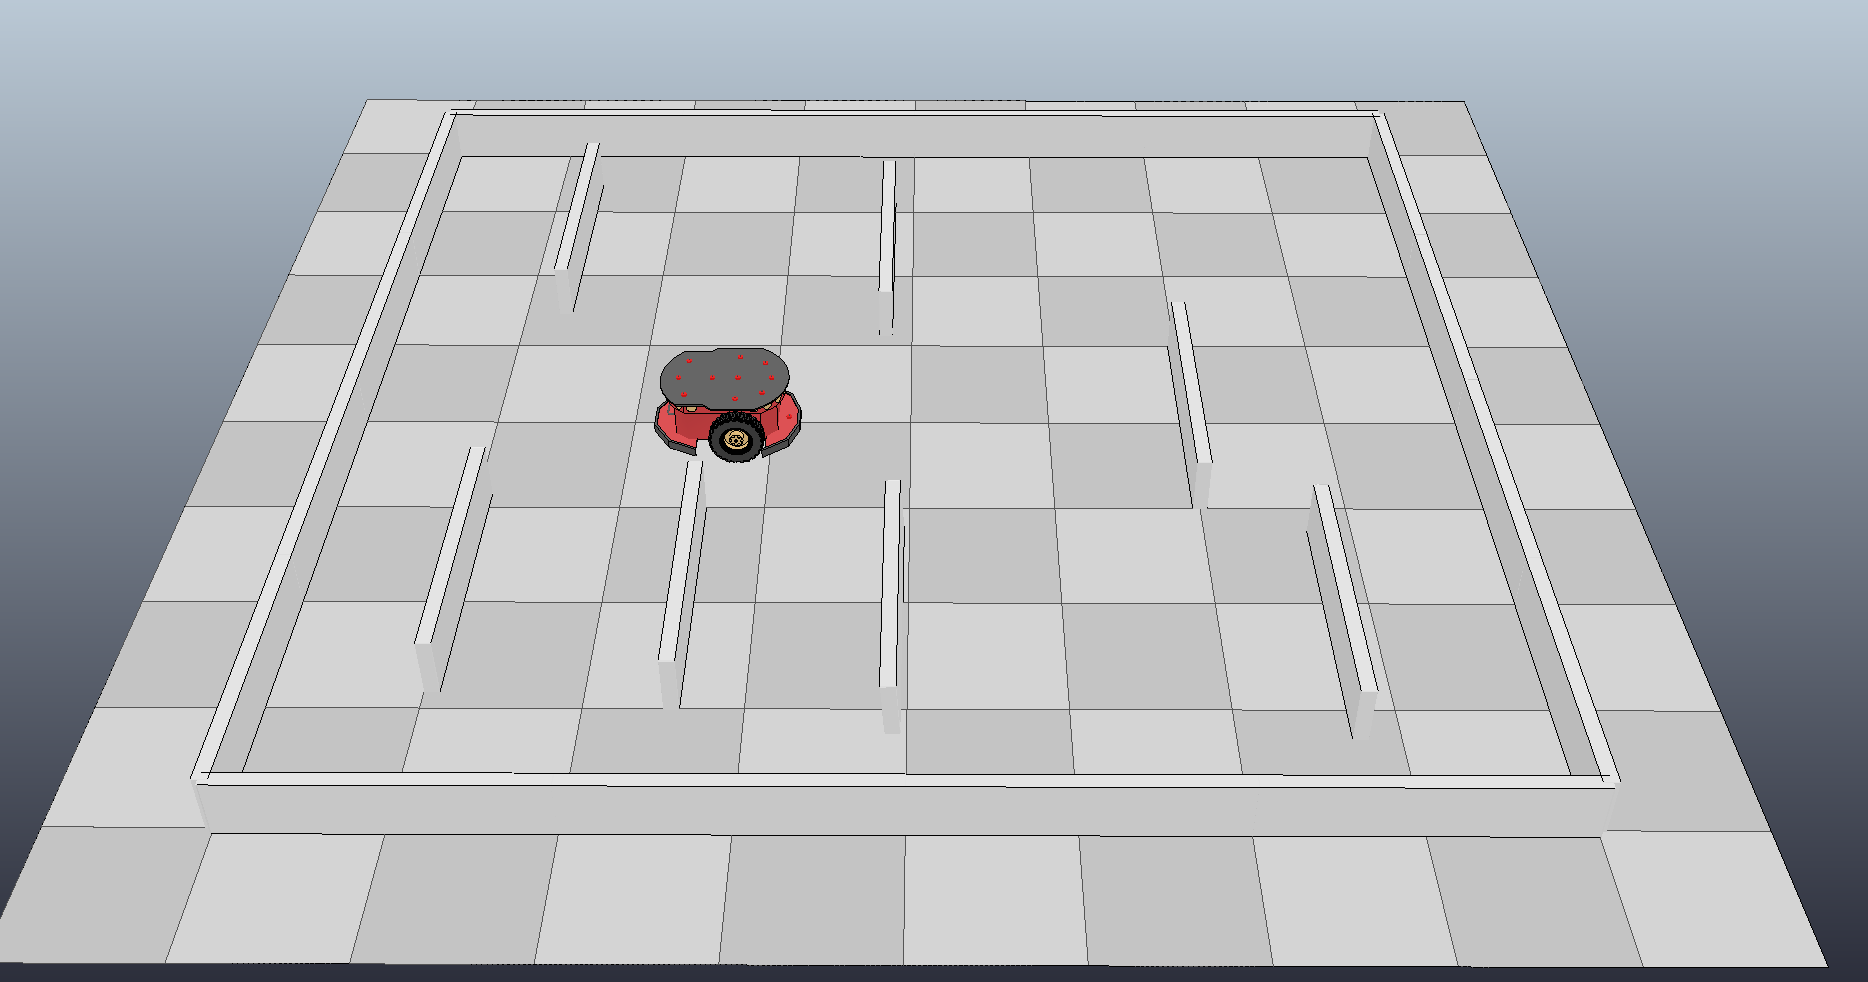
\includegraphics[scale=0.4]{pioneer_labyrinth.png}
\end{center}
\begin{center}
	[Imagen 2: Escenario 1]
\end{center}
En el segundo escenario se ha diseñado un corredor muy sencillo con un ligero giro, y funciona correctamente el controlador final, cumpliendo con el requisito de la práctica.
\begin{center}
	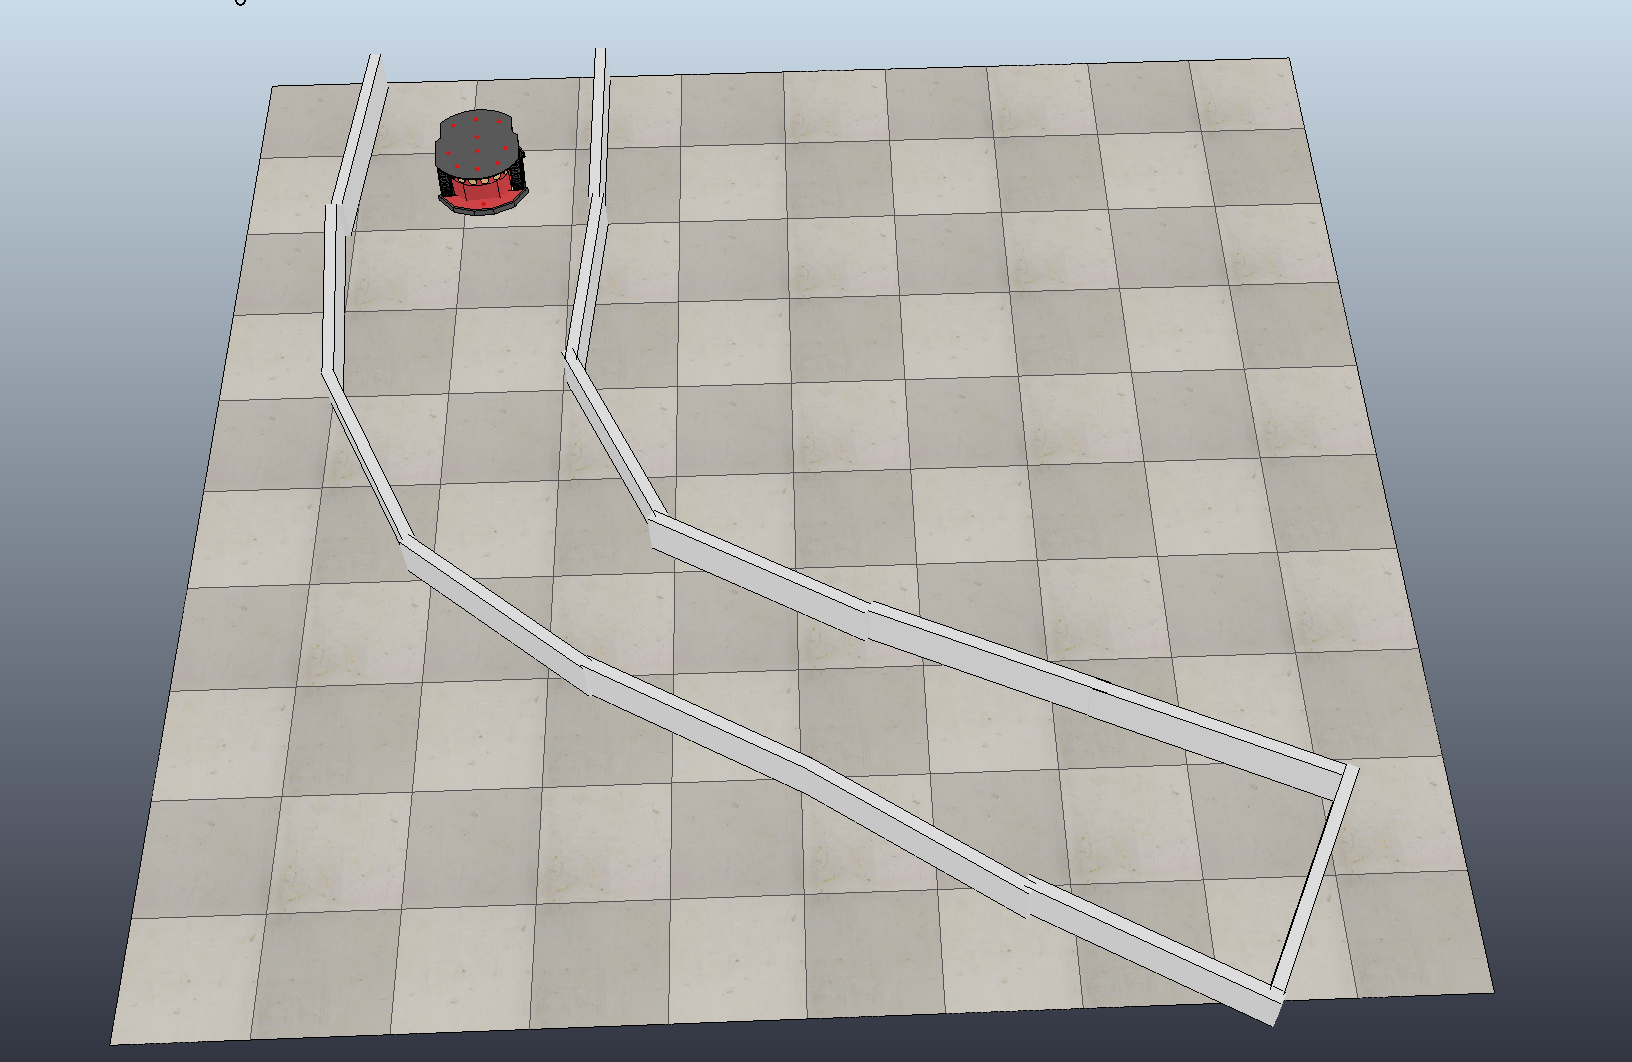
\includegraphics[scale=0.4]{pioneer_corredor.png}
\end{center}
\begin{center}
	[Imagen 3: Escenario 2]
\end{center}
Por último en el escenario tres se añadió un giro más pronunciado para ver el funcionamiento del controlador final, y funcionó correctamente.
\begin{center}
	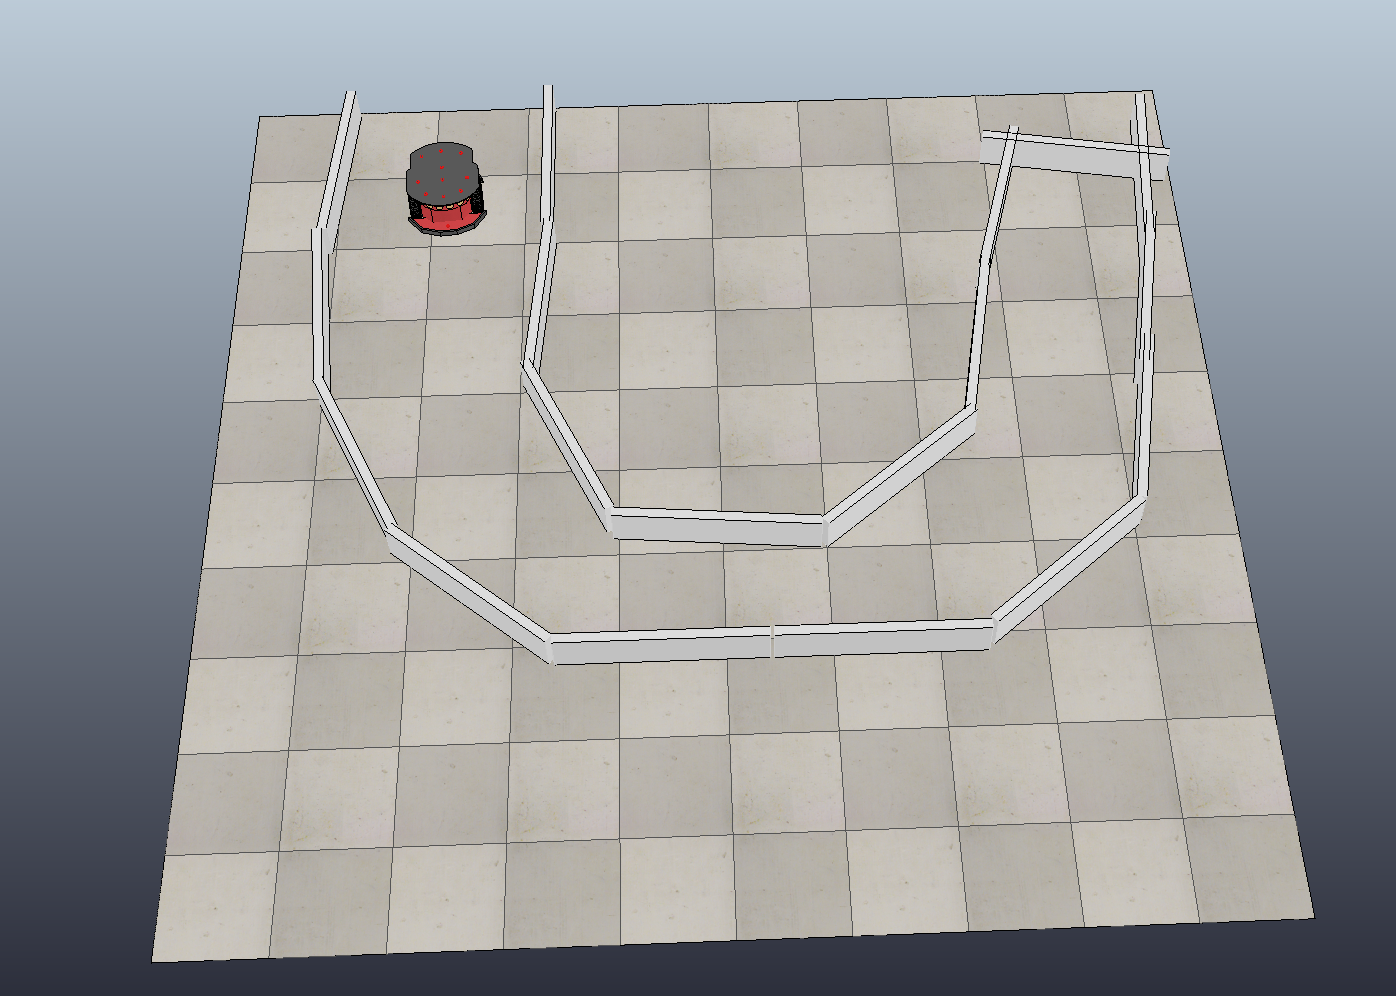
\includegraphics[scale=0.4]{pioneer_corredor_dos.png}
\end{center}
\begin{center}
	[Imagen 4: Escenario 3]
\end{center}
\newpage
\section{Aprendizaje por refuerzo}\label{sec:aprendizajeporrefuerzo}
Finalizando la práctica se ha intentado un modelo de aprendizaje por refuerzo. A continuación explico los problemas que han surgido, las ideas iniciales de lo que se ha querido desarrollar y una primera versión implementada.
\subsection{Ideas iniciales}\label{subsec:ideasiniciales}
El aprendizaje por refuerzo consiste en que el agente aprenda a partir del entorno y genere un controlador para futuras acciones.\\\\
Según el proceso de decisión de Markov (MDP) se tiene un conjunto finito de estados (S), un conjunto de acciones (A) y las interacciones entre ellos. Aquí surgió el primer problema ya que había que modelar este método en un espacio continuo, es decir, una forma de poder decidir que el robot está en un estado cuando este esté en determinado rango del espacio. \\\\
La idea inicial para resolver este problema fue un modelo de estados por rango dirigido por los 16 sensores del robot, limitando el rango al sensor que detectara menor proximidad en cada lado del robot.\\\\
Tendriamos definido el estado actual del robot el conjunto de acciones, y su probabilidad que dependerá de la distancia a un obstáculo, a las que se puede acceder desde el estado sería la dirección (el ángulo) de cada sensor. Por lo tanto el funcionamiento sería el siguiente: se define el estado actual, se elige una dirección y el robot empieza a andar hasta que sale del estado (rango de este); entonces vuelve a definir el nuevo estado y a repetir el proceso.\\\\
La recompensa de un estado será la suma de las distancias a obstáculos de los sensores en ese estado.\\\\
El siguiente problema que se encontró fua al intentar trabajar con Q-Learning ya que hay que inicializar el conjunto de estados, y en este caso los estados son desconocidos (así como su número), por lo tanto simplemente se elimino este paso del algoritmo y ahora cada vez que sale de un estado comprueba si el estado al que ha llegado ya existía o es nuevo.
\subsection{Primera versión}\label{subsec:primeraversion}
La estructura de esta versión para implementar Q-Learning es la siguiente:
\begin{itemize}
	\item S: Estados, array dinámico
	\item A: Acciones, matriz |S| x 16
	\item Q: Q(s, a) Función que devuelve la probabilidad de elegir a estando en el estado s.
\end{itemize}

Se han definido cuatro funciones para realizar el aprendizaje:
\begin{itemize}
	\item getState: devuelve el estado actual a partir de la posición
	\item addNewState: añade un nuevo estado a S
	\item addActionsToState: añade las acciones a un estado
	\item addActionsToQ: añade las probabilidades de las acciones
	\item getReward: obtiene la recompensa de un estado actual a partir de los sensores
\end{itemize}

A falta de terminar la implementación, la idea habría sido ir ejecutando el controlador hasta llegar al final del corredor. Se irían detectando los diferentes estados actuales e ir moviéndose entre estados, haciendo uso de las funciones explicadas arriba. Para añadir un nuevo estado se ha definido el número -1, cuando se detecta que estamos en un estado -1, es que es un nuevo estado.

\newpage
\section{Bibliografía}\label{sec:bibliografia}
\bibliographystyle{plain}
\bibliography{References}
\end{document}
\grid
